\documentclass{report}
\graphicspath{{./img/}}
%************************************************************
% ABOUT THIS HOMEWORK
\def\course{Advanced Data Structures and Algorithms}      %Course
\def\thetitle{Manipulating Bitmap (BMP) images}               % Report Title
\def\Headauthor{Ahmadov Kamal, Osmanli Ravan}         % Header Authors of work
\def\date{\10 May 2023}                             % Date of work

% DOCUMENT START
\begin{document}

% TITLE PAGE
\begin{center}
    \vspace*{1.5cm}
    % University Logo
    
\includegraphics[scale = 0.50]{img/UFAZ.png}\\[1.75cm]
    % University Name
    \textsc{\color[RGB]{0, 51, 102}\LARGE{French-Azerbaijani University}}\\[1cm]
    \textsc{\Large{\course}}\\[.5cm]
    \textsc{\Large{\thetitle}}\\[.5cm]
    \textsc{\date}\\[2cm]
    \Large{
    \begin{tabular}{L{4cm} R{4cm}}
        \textit{Author} &  \textit{Student ID}\\
        \hline
        % author names and PID
        Ahmadov Kamal & 22022692\\
        Osmanli Ravan & 22022753
    \end{tabular}
    }
\end{center}
\thispagestyle{empty}
\pagebreak

% TABLE OF CONTENTS
\tableofcontents{}
\pagebreak

% REPORT START
\section {Introduction}
\begin{introduction}
    Computer-generated images have become indispensable in today's digital era, finding applications in entertainment, advertising, and scientific visualization. Creating visually appealing and unique images is a crucial aspect of computer graphics and image processing. This project focuses on generating customized square images with symmetrical or asymmetrical patterns.

The goal is to develop a program that generates square images according to user-defined specifications, such as size, symmetry type, line thickness, and number of images. By leveraging image manipulation principles and randomization techniques, visually striking patterns can be created.

The project utilizes the BMP (Bitmap) file format, a widely adopted format for storing pixel data. By manipulating the pixel values, the program can generate a diverse range of shapes and patterns.

Implementation-wise, the program is designed using a set of functions and data structures. The \texttt{"image.h"} header file contains the necessary data structures, constants, and function prototypes for image creation, manipulation, and saving. The \texttt{"image.c"} source file houses the function implementations, including initializing image headers, generating pixel data, and saving images in BMP format.

For enhanced usability, the project supports command-line arguments, allowing users to specify output filenames, image sizes, symmetry types, line thickness, and the number of images to generate. Reproducibility of generated images can be ensured by providing an optional seed value.

In subsequent sections, this report will delve into the design and implementation details of the image generation program, including the employed algorithms and overall code structure. Furthermore, sample outputs generated by the program will be showcased, and potential use cases for the generated images will be discussed.

In summary, this project aims to provide a flexible and versatile image generation tool, empowering users to explore and create captivating visual patterns. The program's adaptability extends its applicability across various domains, including art, design, and computer graphics research.
\end{introduction}

\section{Structures and Definitions}

The code includes the following structures and definitions:

\subsection{Enumerations}

\begin{verbatim}
typedef enum {
    AH = 0, // ASSYMETRIC HORIZONTAL
    SH = 1, // SYMMETRIC HORIZONTAL
    AV = 2, // ASSYMETRIC VERTICAL
    SV = 3  // SYMMETRIC VERTICAL
} EDirectionsSymmetry;
\end{verbatim}

This enumeration defines the different directions of symmetry for the generated images. It provides four possible values: \texttt{AH} (Assymetric Horizontal), \texttt{SH} (Symmetric Horizontal), \texttt{AV} (Assymetric Vertical), and \texttt{SV} (Symmetric Vertical).

\subsection{Boolean Definition}

\begin{verbatim}
typedef enum {false, true} bool;
\end{verbatim}

This definition introduces the boolean type with two possible values: \texttt{false} and \texttt{true}.

\subsection{Image Header Structure}

\begin{verbatim}
#pragma pack(push, 1) // exact fit - no padding
typedef struct{
    // BMP Header
    char szType[2]; // "BM"
    u32 nSizeOfFile; // size of file in bytes
    u32 nReserverForApp; // reserved for application. always 0
    u32 nStartOfImage; // offset to start of image data in bytes

    // DIB Header
    u32 nSizeOfHeader; // size of DIB header in bytes
    u32 nWidth; // width of image in pixels
    u32 nHeight; // height of image in pixels
    u16 nNumberOfColorPlanes; // number of color planes. always 1
    u16 nNumberOfBitsPerPixels; // number of bits per pixel

    // Additional information (not necessary for current needs)
    u32 nCompression; // compression method being used (0 = none)
    u32 nSizeOfData; // size of the raw bitmap data in bytes (including padding)
    u32 nResolutionHorizontal; // horizontal resolution of the image (pixel per meter)
    u32 nResolutionVertical; // vertical resolution of the image (pixel per meter)
    u32 nColorsInPalette; // number of colors in the palette 
    u32 nImportantColors; // number of important colors used (0 = all)
} SImageHeader;
#pragma pack(pop) // back to whatever the previous packing mode was
\end{verbatim}

This structure represents the header of the image file, containing information such as the file type, size, image dimensions, color information, and additional metadata.

\subsection{Image Structure}

\begin{verbatim}
#pragma pack(push, 1) // exact fit - no padding
typedef struct{
    unsigned char* pPixels;
    SImageHeader sHeader;
} SImage;
\end{verbatim}

This structure represents the image itself, containing a pointer to the pixel data and the image header.



% Methodology
\section{Methodology}
\label{sec:methodology}

In this section, we describe the methodology used to generate images with specified symmetries. The implementation is based on the provided C code, which consists of several functions and structures for image generation.

\subsection{Image Header Initialization}
The \texttt{SImageInit} function initializes the header of the image. It takes three parameters: \texttt{nWidth} (the width of the image), \texttt{nHeight} (the height of the image), and \texttt{nBitsPerPixel} (the number of bits per pixel). The function creates an instance of the \texttt{SImageHeader} structure and sets its fields according to the provided parameters.

\subsection{Pixel Generation}
The \texttt{ppCreatePixels} function is responsible for generating the pixels of the image. It takes three parameters: \texttt{nSize} (the size of the image), \texttt{nThickness} (the thickness of the line), and \texttt{nDirectionSymmetry} (the direction of symmetry). The function allocates memory for the pixel array and generates random pixel values based on the specified parameters. It also handles the symmetrical copying of pixels if the direction of symmetry is set to either symmetric horizontal or symmetric vertical.

\subsection{Image Creation}
The \texttt{createImage} function combines the image header initialization and pixel generation to create the final image. It takes several parameters: \texttt{nWidth} (the width of the image), \texttt{nHeight} (the height of the image), \texttt{nBitsPerPixel} (the number of bits per pixel), \texttt{pPixels} (the pixel array), \texttt{nDirectionSymmetry} (the direction of symmetry), and \texttt{nThickness} (the thickness of the line). The function initializes the image header, allocates memory for the pixel data, fills the image with white pixels, and draws the specified line according to the provided parameters.

\subsection{Image Saving}
The \texttt{saveImage} function is responsible for saving the generated image to a file. It takes two parameters: \texttt{image} (the image structure) and \texttt{szFileName} (the name of the file). The function opens the file in binary write mode, writes the image header to the file, followed by the pixel data, and finally closes the file.

\subsection{Image Generation}
The main function serves as the entry point of the program. It processes command-line arguments to determine the output file name, image size, symmetry direction, and other parameters. It then generates the specified number of images by calling the \texttt{createImage} and \texttt{saveImage} functions. The random seed for image generation can be optionally specified through the command-line argument or set to the current time.

\subsection{Command-Line Arguments}
The program supports various command-line arguments to customize the image generation process. The available arguments are:

\begin{itemize}
  \item \texttt{-o <output file name>} specifies the output file name for the generated image.
  \item \texttt{-size <size of the image>} sets the size of the image (width and height).
  \item \texttt{-n <number of images to be generated>} specifies the number of images to generate.
  \item \texttt{-seed <seed for random number generator>} sets the seed for the random number generator used in image generation.
  \item \texttt{-ah}, \texttt{-av}, \texttt{-sh}, \texttt{-sv} specify the direction of symmetry for the image. \texttt{-ah} represents horizontal asymmetry, \texttt{-av} represents vertical asymmetry, \texttt{-sh} represents symmetric horizontal, and \texttt{-sv} represents symmetric vertical.

\end{itemize}

\subsection{Example Usage}
Here is an example usage of the command-line arguments to generate images with various symmetries:

\begin{verbatim}
$ ./symasym -o output -size 100 -n 10 -sh 
\end{verbatim}

This command generates 10 images with a size 100x100 pixels with the output name starting with "output"The images have symmetric horizontal symmetry and a line. 

\subsection{Conclusion}
In this section, we have described the methodology used for generating images with specified symmetries. We discussed the image header initialization, pixel generation, image creation, image saving, and command-line arguments. The provided C code implements these functionalities to generate images with various symmetries.

\section{Design and Implementation}

In this section, we will discuss the design and implementation details of the image generation program. The program consists of three main components: the image header definition, the image creation functions, and the main program logic.

\subsection{Image Header Definition}

The image header is defined in the \texttt{image.h} header file. It includes the necessary definitions and structures to represent the BMP header and DIB header of the image. The \texttt{SImageHeader} structure contains fields such as the file size, image dimensions, color information, compression method, and other relevant details. It is defined using a packed structure to ensure that there is no padding between the fields.

\subsection{Image Creation Functions}

The image creation functions are implemented in the \texttt{image.c} source file. These functions provide the necessary functionality to generate the image pixels and create the image. 

The \texttt{SImageInit} function initializes the image header with the specified width, height, and bits per pixel. It sets the appropriate values for the BMP header and DIB header fields.

The \texttt{ppCreatePixels} function generates the pixels of the image based on the specified size, line thickness, and direction of symmetry. It allocates memory for the pixel array and fills it with randomly generated pixel values. If the symmetry is enabled, it copies the pixels to the other half of the image.

The \texttt{createImage} function creates the image using the provided image dimensions, bits per pixel, pixel array, direction of symmetry, and line thickness. It initializes the image header using \texttt{SImageInit}, allocates memory for the pixel data, and fills it with the appropriate pixel values based on the line positions and symmetry.

The \texttt{saveImage} function saves the generated image to a BMP file. It takes the image structure and the output file name as parameters, opens the file in binary write mode, and writes the image header and pixel data to the file. Finally, it closes the file.

\subsection{Main Program Logic}

The main program is implemented in the \texttt{symasym.c} source file. It handles the command-line arguments, generates the specified number of images, and saves them to BMP files. The program parses the command-line arguments to extract the output file name, image size, symmetry options, number of images, and random seed if specified. It then iterates over the number of images, generating a unique seed for each iteration and using it to generate the image with the specified symmetry. The image is saved to a BMP file with a suffix indicating the symmetry and the seed value.

\subsection{Usage}

The program can be executed with various command-line arguments to customize the image generation process. The available options include specifying the output file name, image size, symmetry direction, number of images, and random seed. For example:

\texttt{\$ ./symasym -o output -size 64 -sh -n 5}

This command generates 5 images with a size of 64x64 pixels, horizontal symmetry, and saves them to files named \texttt{outputshXXXX.bmp}, where \texttt{XXXX} represents the seed value.

The program provides flexibility in generating images with different sizes, symmetries, and random seeds, allowing users to generate a variety of images for their needs.

\subsection{Summary}

In summary, the image generation program consists of the image header definition, image creation functions, and the main program logic. The image header provides the necessary structure to represent the BMP and DIB headers. The image creation functions generate the image pixels and create the

\section{Examples of Generated Images}

The following examples demonstrate the output images generated by the command \texttt{./symasym -size 100 -sv -n 5}. Each image is a square of size 100x100 pixels with vertical symmetry.

\begin{figure}[htbp]
  \centering
  \begin{tabular}{ccccc}
    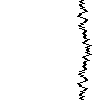
\includegraphics[width=0.18\linewidth]{img/sv1684184414.png} &
    
\includegraphics[width=0.18\linewidth]{img/sv1684184415.png} &
    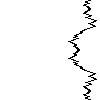
\includegraphics[width=0.18\linewidth]{img/sv1684184416.png} &
    
\includegraphics[width=0.18\linewidth]{img/sv1684184417.png} &
    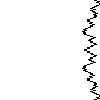
\includegraphics[width=0.18\linewidth]{img/sv1684184418.png} \\
    (a) Image 1 & (b) Image 2 & (c) Image 3 & (d) Image 4 & (e) Image 5 \\
  \end{tabular}
  \caption{Examples of images generated with vertical symmetry}
  \label{fig:examples}
\end{figure}

As shown in Figure \ref{fig:examples}, each image exhibits vertical symmetry, where the left half of the image is a mirror reflection of the right half. The generated images showcase variations in line thickness, positions, and the overall appearance due to the random nature of the generation algorithm.

These examples illustrate the versatility and flexibility of the image generation process, allowing for the creation of unique and visually interesting patterns with different settings and symmetries.

\section {Conclusion}

In this project, we have developed a program for generating square images with specified symmetries using the BMP (Bitmap) file format. The program allows users to customize various parameters such as image size, symmetry type, line thickness, and the number of images to generate.

By leveraging image manipulation principles and randomization techniques, visually striking patterns can be created. The program utilizes functions and data structures to handle image header initialization, pixel generation, image creation, and image saving. It supports command-line arguments for enhanced usability and reproducibility.

The generated images can find applications in various domains, including art, design, and computer graphics research. The program's flexibility and adaptability empower users to explore and create captivating visual patterns.

In conclusion, the developed image generation program provides a versatile tool for creating customized square images with symmetrical or asymmetrical patterns, contributing to the field of computer graphics and image processing.


%************************************************************
\end{document}